% -*- root: ../main.tex -*-
\chapter{Implementazione}
\section{Microcontrollori}
\subsection{Battito Cardiaco}
Un parte particolarmente complessa è stata quella della modellazione del sensore per il battito. Il sensore, qualora interpellato, fornisce un singolo valore direttamente proporzionale alla dilatazione dei vasi sanguigni. Ne deriva la necessità di attuare misurazioni frequenti per non incorrere nella perdita della breve variazione di un battito. Abbiamo stabilito la frequenza di campionamento in base a quanto segue:
Considerando che in condizioni di riposo, i battiti per minuto di un cane - da intendersi come pulsazioni - sono generalmente compresi tra 60 e 140 bpm, in base alla taglia, età e razza, e il valore può raggiungere valori anche più alti qualora in movimento, abbiamo preso come valore limite da rilevare 150 bpm. Ciò, significa che il tempo di ogni ciclo cardiaco $T_{cc}$ è:
\begin{equation}
T_{cc} = \frac{1}{bps} = \frac{1}{\frac{bpm}{60}}= \frac{60}{bpm} \Rightarrow \frac{60}{150 bpm} = 0.4s
\end{equation}
Considerato che il ciclo cardiaco si compone in sistole (contrazione) e diastole (rilassamento), la fase sistolica è quella più facilmente rilevabile poichè la contrazione ventricolare causata è più violenta e breve. Questa fase durante le rilevazioni effettuate dura circa un mezzo del ciclo cardiaco e produce un picco nei valori particolarmente indicativo per rilevare il battito in mezzo al naturale rumore del sensore. Per non perdere il picco massimo il numero di campionamenti $N_{c}$ durante questa fase è stato fissato a 20. La frequenza di campionamento minima risultante $f_{min}$ è stata calcolata come: 
\begin{equation}
f_{min} = \frac{ \frac{1}{2} *  T_{cc} }{N_{c}} \Rightarrow  \frac{ \frac{1}{2} *  0.4s }{20} = 0.01s = 10 ms 
\end{equation}

Salvando i valori risultanti e graficandoli con la libreria python "Mathplotlib" si ottiene una linea come quella di colore rosso in [Fig. \ref{fig:Heartbeat}]. Si può notare che il campionamento è sufficiente e permette di distinguere intuitivamente i battiti. 
Per rilevare le pulsazioni a livello digitale però è necessario formalizzare un altro modello matematico che non faccia incorrere il sistema in falsi positivi o falsi negativi. Un primo approccio si è basato su stabilire una singola soglia, oltre la quale il battito è rilevato e registrato. Questa soluzione si è rivelata inadatta in quanto il disturbo del sensore la farebbe attraversare più volte (si veda in [Fig. \ref{fig:Heartbeat}] poco prima del campionamento numero 2400 il valore attraversa la linea azzurra parecchie volte). Inadatti si sono rivelati anche i tentativi di normalizzare la linea dei valori, in quanto parecchio discontinui e di frequenza elevata, si perde la differenziazione dei picchi. Si è optato per stabilire una doppia soglia, la prima, più alta, oltre la quale il battito è rilevato, la seconda, più bassa, che determina la fine del battito. La prima volta che il valore attraversa la prima [Fig. \ref{fig:Heartbeat}, linea azzurra] una variabile registra il battito e nessun altra registrazione viene effettuata sino a che i valori non scendono sotto la soglia di fine battito [Fig. \ref{fig:Heartbeat}, linea gialla]. 
Queste soglie non possono essere fisse, variando la pressione di animale in animale e pure di giorno in giorno per lo stesso essere vivente. Per questo motivo i valori sono stati fissati per la prima a 4/5 e per la seconda a 1/2 tra minimo [Fig. \ref{fig:Heartbeat}, linea verde] e massimo [Fig. \ref{fig:Heartbeat}, linea blu] dei precedenti valori. La grandezza della finestra dei valori da cui prendere minimo  e massimo è stata fissata a 250 valori. Questo perchè, come si può notare dal grafico, comprende almeno due battiti. Un range troppo piccolo creerebbe dei minimi e massimi locali, rilevando picchi non propri e dando parecchi falsi positivi. Una finestra troppo ampia porterebbe a una staticità delle soglie rispetto alla variazione di pressione che creerebbe falsi negativi.  

    %GRAFICO BATTITO
    \begin{figure}[H]
        \caption{Grafico Battiti}
        \label{fig:Heartbeat}
        \centering
        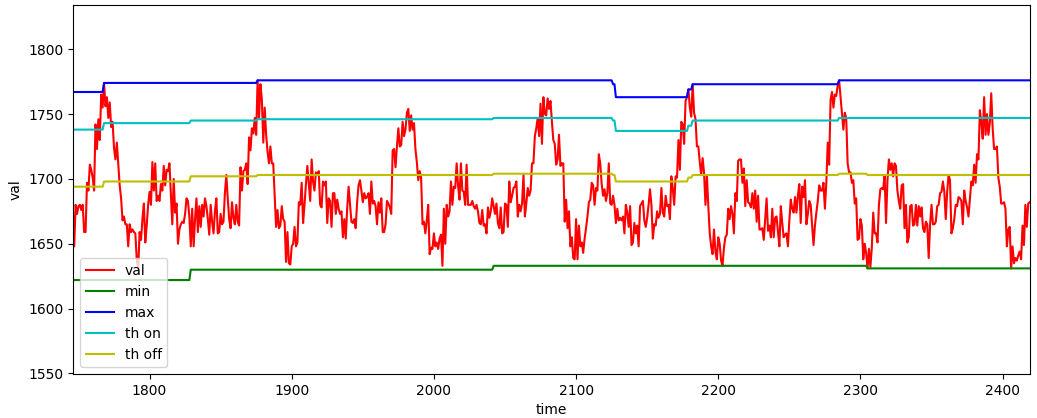
\includegraphics[width=1\textwidth]{Images/heartbeatGraph.png}
    \end{figure}

Una volta rilevati i singoli battiti con il modello matematico, il calcolo del battiti al minuto è stato realizzato salvando la cronologia degli istanti di tempo per gli ultimi N battiti $N_{beats}$. Sperimentalmente si è optato per 30 registrazioni per mantenere il valore dei bpm reattivo ma non dipendente solo da poche unità. Prelevando dalla cronologia il tempo passato $T_{diff}$ per questi battiti, si può facilmente derivare il rateo di $bpm$ attuale tramite la formula: 
\begin{equation}
bpm = \frac{ N_{beats}*60 s/min }{T_{diff}} = \frac{ N_{beats}*60 s/min }{T_{last}-T_{first}} 
\end{equation}
Il battito cardiaco risultante viene poi inviato periodicamente al Database e, qualora ci fossero anomalie, una notifica viene invece generata e inviata immediatamente.
\begin{tcolorbox}[tab2,tabularx={c||c|c|Y|Y},title=Confronto Prestazioni Microcontrollori Testati,boxrule=0.5pt] \hline
board & velocità processore & costo & tempo medio avvio programma & tempo medio connessione MQTT \\ \hline
\hyperlink{https://en.wikipedia.org/wiki/ESP8266}{ESP8266} & 160 MHz & 5€ & 8,1 s & 9,3 s\\ \hline
\hyperlink{https://en.wikipedia.org/wiki/ESP32}{ESP32} & 240 MHz (dual core) & 7€ & 5,2 s & 3,4 s\\ \hline
\end{tcolorbox}

\input{Tex/Implementation/SaraKiade}
\input{Tex/Implementation/GyordanCaminati}
